\section{Mechanical Model}\label{sec:neuro_mech_model}

To obtain the simulation results we present in \cref{sec:control_sim}, we
construct a mechanical model in the Matlab Simscape Multibody environment
similar to those presented in \citet{geyer2010muscle, song2013integration,
song2015neural}. This model represents the seven link biped in
\cref{fig:neuro_seven_link} and includes two legs with thigh, shank, and foot
segments as well as a lumped head-arms-trunk (HAT) segment.
\Cref{tab:model_mech_params} lists the segment lengths, center of mass and joint
locations measured from the distal end, masses, and inertias that approximate
those of a \unit[80]{kg}, \unit[1.8]{m} tall person.

\begin{table}[b]
  \centering
      \begin{tabular}{lcccc}
        \toprule
        & Feet & Shanks & Thighs & HAT \\
        \midrule
        $l         \ (\unit{cm})$ & 20    & 50   & 50   & 80   \\
        $d_\tn{COM}   \ (\unit{cm})$ & 14    & 30   & 30   & 35   \\
        $d_\tn{Joint} \ (\unit{cm})$ & 16    & 50   & 50   &      \\
        $m         \ (\unit{kg})$ & 1.25  & 3.5  & 8.5  & 53.5 \\
        $J         \ (\unit{kg})$ & 0.005 & 0.05 & 0.15 & 3    \\
        \bottomrule
      \end{tabular}
  \caption{Segment lengths $(l_s)$, center of mass $(d_\tn{COM})$ and joint
  $(d_\tn{Joint})$ locations measured from the distal end, masses $(m)$, and
  inertias $(J)$ approximated from
  \citet{gunther2003synthesis}.}\label{tab:model_mech_params}
\end{table}

The mechanical model interacts with the environment through ground reaction
forces on the toes and balls of the feet. Specifically, we use a 2-dimensional
reduction of the 3D ground contact model presented in
\citet{song2013generalization} to calculate forces in the normal and
tangential directions with respect to the terrain. In the normal direction the
force is
\begin{align}
    F_\tn{n} = k_\tn{n} \Delta n_\tn{c} (1 + \dot n_\tn{c}) 
        (\Delta n_\tn{c} > 0)
    \left(\nicefrac{\dot n_\tn{c}}{v_\tn{max}} > -1 \right),
    \label{eq:grf_n}
\end{align}
where $k_\tn{n} = \unitfrac[78.45]{N}{mm}$ is the stiffness coefficient in the
normal direction and $\Delta n_\tn{c}$ and $\dot n_\tn{c}$ are the penetration
direction and velocity in the normal direction. The form of the normal force is
inspired by \citet{gunther2003synthesis} and \citet{scott1993biomechanical} and
represents a linear spring with multiplicative damping.  $v_\tn{max} =
\unitfrac[3]{cm}{s}$ represents the maximum recovery velocity of the ground. If
$\dot n_\tn{c}$ exceeds this velocity, ground contact is lost.

In the tangential direction, a state machine switches between two force models
representing sliding and static friction. Sliding friction is given by
\begin{align}
    F_{\tn{t,slide}} = -\func{sign}{\dot t_\tn{c}} \mu_\tn{slide} F_\tn{n}
\end{align}
while static friction is given by
\begin{align}
    F_{\tn{t,static}} = -k_t \Delta t_c \left(1 + \func{sign}{\Delta t_c}
    \frac{\dot t_c}{v_\tn{max}} \right),
\end{align}
where $\Delta t_c$ is the penetration in the tangential direction $\dot t_c$ is
the penetration velocity, $\mu_\tn{slide} = 0.8$ is the sliding coefficient of
friction, and $k_\tn{t} =\unitfrac[78.45]{N}{mm}$ is the stiffness coefficient
in the tangential direction.

The contact model begins in the sliding mode and switches to the static mode if
$\dot t_\tn{c} < \unitfrac[1]{cm}{s}$. It switches back to the sliding mode when
$| F_{\tn{t,static}} | < \mu_\tn{static} | F_\tn{n} |$, where $\mu_\tn{static} =
0.9$.

Finally, the biped skeletal model includes soft joint limits to represent
the skeletal joint limits on the knee, ankle, and hip joints. The functional
form form the soft limit joint torque is identical to that of the normal ground
reaction force given by \cref{eq:grf_n}.
\begin{align}
    \tau_\tn{jl} = k_\tn{jl} \Delta \phi_\tn{jl} (1 + \dot \phi_\tn{jl}) (\Delta
    \phi_\tn{jl}  > 0) \left(\nicefrac{\dot \phi_\tn{jl}}{\dot \phi_\tn{max}} > -1
    \right), 
    \label{eq:tau_joint_limit}
\end{align}
where $k_\tn{jl} = \unitfrac[0.3]{N \cdot m}{deg}$ is the joint stiffness $\Delta
\phi$ and $\dot \phi_\tn{jl}$ are the joint limit penetration angle and
velocity respectively, and $\dot \phi_\tn{max} = \unitfrac[1]{deg}{s}$ is the
maximum joint limit retraction velocity. \Cref{tab:joint_lim} lists the
engagement angles for the joint limits.
\begin{margintable}[-0.65in]
  \centering
      \begin{tabular}{lcc}
        \toprule
        Joint & ext.\ lim.\ & flex lim.\ \\
        \midrule
        hip   &     & 50 \\
        knee  &   5 &    \\
        ankle & -40 & 20 \\
        \bottomrule
      \end{tabular}
  \caption{Joint limits for the hip, knee, and ankle joints listed in degrees.
  Positive joint angles represent flexion and negative joint angles represent
  extension (see \cref{fig:neuro_seven_link}).}\label{tab:joint_lim}
\end{margintable}

To obtain simulation results, we simulate the mechanical system with the
\verb+ode15s+
variable step solver. We set the maximum step size to $\unit[10]{ms}$, relative
error tolerance to $10^{-4}$, and abolute error to $10^{-6}$.

\section{Hill Muscle Models}\label{sec:neuro_hill_muscle}
\begin{marginfigure}[-0.25in]
    \centering
    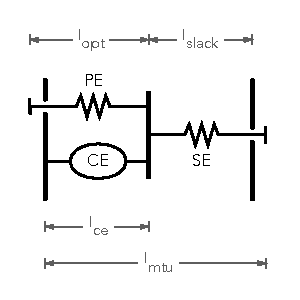
\includegraphics[width=\linewidth]{mtu_figure}
    \vspace{-0.4in}
    \caption{Hill-type muscle tendon unit with contractile element (CE),
    parallel elasticity (PE), and series elasticity (SE).}
    \label{fig:hill_type_mtu}
\end{marginfigure}
Our proposed transfemoral prosthesis control is comprised of biological muscle
actuators that are stimulated according to hypothesized reflex pathways.
Specifically, we use a Hill-type \emph{muscle tendon unit} (MTU) first described
by \citet{hill1938heat}. It is comprised of a contractile element (CE) that
represents muscle fibers and produces force when activated, a parallel elastic
(PE) element that represents the stiffness of the collagen tissue between muscle
fascicles, and series elastic (SE) element that models tendon stretch.
\Cref{fig:hill_type_mtu} shows the arrangement of these elements. Note that the
PE and SE both are unidirectional springs with engagement lengths of
$l_\tn{opt}$ and $l_\tn{slack}$ respectively.

The CE generates force according to
\begin{align}
    F_\tn{CE} = F_\tn{max} A \func{f_l}{l_\tn{CE}} \func{f_v}{v_\tn{CE}}.
    \label{eq:hill_ce}
\end{align}
In this equation, the force generated by the CE, $F_\tn{CE}$, is the maximum
isometric (constant length) force, $F_\tn{max}$, multiplied by activation, $A$,
the force-length, $\func{f_l}{\cdot}$, and force-velocity, $\func{f_v}{\cdot}$,
relationships of the CE\@. The activation, $A$, is a low-pass filtered version
of the stimulation signal muscle $S(t)$ generated by the muscle reflexes we will
detail in the \hyperref[sec:neuro_stance_reflexes]{next} section. This filter,
given by $A(t) = S - \tau \dot A(t)$ with time constant $\tau$, represents the
diffusion dynamics of calcium ions that activate binding sites in the muscle
fibers.
\begin{marginfigure}[-1in]
    \centering
    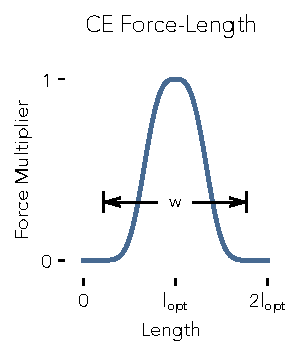
\includegraphics[width=\linewidth]{force_length_ce_annotate}
    \vspace{-0.25in}
    \caption{Force-length relationship of the CE.}
    \label{fig:force_length_ce}
\end{marginfigure}

The binding sites are where overlapping actin and myosin filaments attach and
generate pulling force. The contractile element length of $l_\tn{opt}$
corresponds to maximum overlap between these filaments. Therefore, as as the
muscle length moves away from $l_\tn{opt}$, its force production capacity
decreases leading to the force-length relationship shown in
\cref{fig:force_length_ce}. We model the force-length relationship via a bell
curve
\begin{align}
    \func{f_l}{l_\tn{CE}} = \exp \left( \ln(0.05) \left|
    \frac{l_\tn{CE} - l_\tn{opt}}{w l_\tn{opt}}
    \right|^3 \right).
    \label{eq:hill_force_length}
\end{align}
\begin{marginfigure}[0.25in]
    \centering
    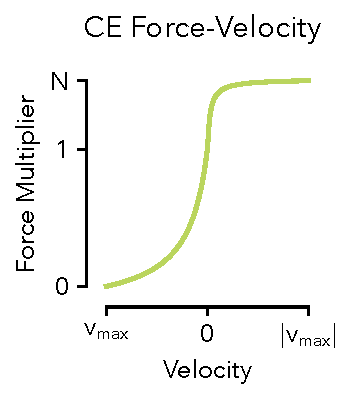
\includegraphics[width=\linewidth]{force_velocity_ce}
    \vspace{-0.25in}
    \caption{Force-velocity relationship of the CE.}
    \label{fig:force_velocity_ce}
\end{marginfigure}

The velocity-dependent filament attachment probabilities give rise to a
force-velocity relationship shown in \cref{fig:force_velocity_ce}. The following
expression captures this relationship.
\begin{table}[t]
  \centering
  \begin{tabular}{lc|lc}
    \toprule
    Param & Value             & Param                   & Value \\
    \midrule                           
    $\tau$ & \unit[0.01]{s}   & $l_\tn{opt}^\tn{ham}$   & \unit[0.10]{m} \\
    $w$    & 0.56             & $v_\tn{max}^\tn{ham}$   & \unitfrac[-1.2]{m}{s} \\
    $K$    & 5                & $F_\tn{max}^\tn{ham}$   & \unit[3000]{N} \\
    $N$    & 1.5              & $l_\tn{slack}^\tn{ham}$ & \unit[0.31]{m} \\
    $\epsilon_\tn{PE}$ & $w$  &                         & \\
    $\epsilon_\tn{SE}$ & 0.04 &                         & \\
    \bottomrule
  \end{tabular}
  \caption{Neuromuscular parameters for shared entities (left) and the hamstring
  muscle (right)}
  \label{tab:neuromusc_params}
\end{table}
\begin{align}
    \func{f_v}{v_\tn{CE}} = 
    \begin{cases} 
        \frac{v_\tn{max} - v_\tn{CE}}{v_\tn{max} + K v_\tn{CE}}, 
            & \textrm{if } v_\tn{CE}< 0 \\
        N + (N-1) \frac{v_\tn{max} + v_\tn{CE}}{7.56 K v_\tn{CE} - v_\tn{max}}, 
            & \textrm{if } v_\tn{CE} \ge 0 
    \end{cases}
\end{align}
In this expression, $K$ is a shape parameter and $N$ determines the force
amplification when the contractile element is lengthening. The force-velocity
relationship acts as a multiplicative damper causing the CE to produce more
contractile force when it is lengthening and less as it contracts.

We model both passive elements, the PE and SE, using the same functional form
representing a unidirectional, stiffening spring, the behavior of which is shown
in \cref{fig:force_length_pese}. The expressions for the elastic force produces
by these elements are
\begin{align}
    \func{F_\tn{PE}}{l_\tn{CE}} &= F_\tn{max} \left( \frac{l_\tn{CE} -
        l_\tn{opt}}{\epsilon_\tn{PE} l_\tn{opt}} \right)^2 
        (l_\tn{CE} > l_\tn{opt}) \label{eq:parallel_force_length}\\
    \func{F_\tn{SE}}{l_\tn{SE}} &= F_\tn{max} \left( \frac{l_\tn{SE} - 
        l_\tn{slack}}{\epsilon_\tn{SE} l_\tn{slack}} \right)^2 
        (l_\tn{SE} > l_\tn{slack}). \label{eq:series_force_length}
\end{align}
\begin{marginfigure}
    \centering
    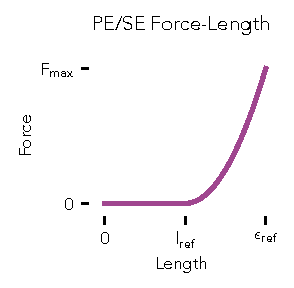
\includegraphics[width=\linewidth]{force_length_pese}
    \caption{PE and SE force length relationship. For the PE, $l_\tn{ref} = l_\tn{opt}$
    and $\epsilon_\tn{ref} = \epsilon_\tn{PE}$. Likewise, for the SE, $l_\tn{ref} =
    l_\tn{slack}$ and $\epsilon_\tn{ref} = \epsilon_\tn{SE}$.} 
    \label{fig:force_length_pese}
\end{marginfigure}

The left-hand side of \cref{tab:neuromusc_params} lists the parameters common
among all seven muscles of each leg of the neuromuscular model. On the
right-hand side of the table, we list four muscle-specific parameters for
hamstrings muscle. For a complete list of muscle parameters please refer
to \citet{song2015neural}. 

\begin{figure}[b]
    \centering
    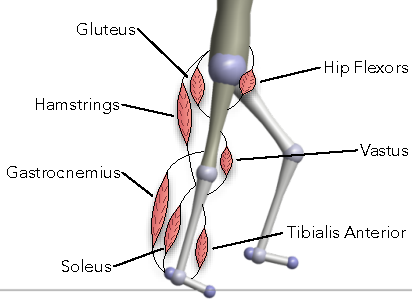
\includegraphics[width=3in]{biped_w_muscles}
    \caption{Biped walking model with labeled muscles.} 
    \label{fig:biped_w_muscles}
\end{figure} 
The full biped model, shown in \cref{fig:biped_w_muscles}, includes
seven Hill-Type muscle-tendon units: soleus, gastrocnemius, tibialis anterior,
vastus, hamstring, hip flexors, and gluteus. The length of these MTUs is related
to the joint angles according to the variable-length moment arms
$\func{r}[\tn{mtu}][j]{\phi^j}$ for each muscle about each joint. For example,
the length of a biarticular muscle spanning joints $j$ and $k$ is
\begin{align}
    l_\tn{mtu} = l_\tn{opt} + l_\tn{slack} + \rho \left( \int_{\phi_0^j}^{\phi^j}
        \func{r}[\tn{mtu}][j]{\phi^j} \tn{d} \phi^j + \int_{\phi_0^k}^{\phi^k}
        \func{r}[\tn{mtu}][k]{\phi^k} \tn{d} \phi^k \right).
\end{align}
Where $\rho$ is a parameter that approximates the effect of the pennation angle 
of the muscle fibers. The variable length moment arms also govern the torque a
muscle produces about a joint according to
\begin{align}
    \tau_\tn{mtu} = \func{r}[\tn{mtu}][j]{\phi^j} F_\tn{mtu}.
    \label{eq:muscle_moment}
\end{align}
